\documentclass[12pt]{article}

\usepackage{hyperref}
\usepackage{graphicx}
\usepackage{enumitem}
\usepackage{xepersian}

\settextfont{Vazirmatn}
\linespread{1.3}

\author{متین اعظمی}
\author{محمد حسینی}
\author{عسل خائف}
\author{ارشیا شفیعی}
\author{شیدا عابدپور}
\author{امیرعلی لطفی}
\author{زهرا معصومی}
\title{سامانه کارا}

\begin{document}

	\begin{figure}
		\centering
		
\includegraphics[width=0.3\textwidth]{files/logo}
	\end{figure}
	\begin{center}
		دانشگاه اصفهان\\
		دانشکده مهندسی کامپیوتر
		\vspace{2\baselineskip}

		{\Huge \textbf{سامانه کارا}}\\

		\vspace{1\baselineskip}
		کاریابی هدفمند در سازمان‌ها، شرکت‌ها و صنایع\\
		\vspace{2\baselineskip}
		\textbf{پدیدآورندگان به ترتیب الفبا:}\\
		متین اعظمی\\
		محمد حسینی\\
		عسل خائف\\
		ارشیا شفیعی\\
		شیدا عابدپور\\
		امیرعلی لطفی\\
		زهرا معصومی\\

		\vspace{1\baselineskip}
		{\textbf{استاد راهنما:}}
		 دکتر محمدرضا شعرباف\\
		\vspace{2\baselineskip}
		ترم پاییز 1401

	\end{center}
	\newpage
	\tableofcontents
	\newpage

	\section{سند تبیین نیازمندی‌ها}

	\subsection{مقدمه}
	در این بخش به تبیین نیازمندی‌های سیستم می‌پردازیم که در قالب استاندارد 1998-830
	\textbf{\lr{Std IEEE}}
	 بیان شده است.
	با توجه به افزایش روز افزون مسئله کاریابی، نیاز به بستری برای تسهیل و تسریع این فرایند حس می‌شود. بدیهی است که مدیریت این فرایند و اطمینان یافتن از درست طی شدن آن نیاز به برنامه‌ریزی دقیقی دارد.
	در این پروژه سامانه‌ای طراحی شده است که علاوه بر کمک به کارجویان جهت کاریابی آسان‌تر و جلوگیری از مراجعه حضوری به دفاتر کاریابی و استفاده از روش‌های سنتی، کمک به کارفرمایان جهت استخدام دقیق و بهتر کارجویان خود را در نظر داشته باشد.


	\subsubsection{هدف}
	سند تبیین نیازمندی‌های نرم‌افزار و یا به اختصار
	\textbf{SRS}
	، سندی است که در آن به شرح کامل جزئیات نیازمندی‌های سیستم، طریقه ارتباط آنها با سیستم و یا با یکدیگر، عوامل تاثیرگذار بر سیستم، واسط‌های گوناگونی که در بخش‌های مختلف سیستم به کار رفته است و کارکرد محصول از جنبه‌های مختلف می‌پردازد.
	به طور خلاصه، این سند دیدی جامع از محصول را به نمایش می‌گذارد و به سه گروه از افراد کمک می‌کند و نیازمندی‌های آن‌ها به دست آمده است:

	\begin{enumerate}
		\item
		\textbf{کارجویان:}
		این سند نشان‌ دهنده آن است که کارجو از سیستم چه انتظاراتی دارد و چه نیازمندی‌هایی باید برای این انتظارات در نظر گرفته شود. این کار باعث شده کارجو درک بهتری از نیازهای خود پیدا کرده و نیازهایش را مدیریت کند.
		\item
		\textbf{کارفرمایان:}
		این سند نشان دهنده آن است که کارفرما از سیستم چه انتظاراتی دارد و جهت تسهیل و تسریع روند استخدام چه نیازمندی‌هایی باید برای او در نظر گرفته شود. این کار باعث شده کارفرما درک بهتری از نیاز‌های خود پیدا کرده و آن‌ها را مدیریت کند.
		\item
		\textbf{مدیر سیستم:}
		این دسته از افراد نیز همانند کارجویان و کارفرمایان، باید دید کلی و جامعی از نیازمندی‌های سیستم داشته باشند. لذا این سند یک توافق اولیه میان کارجو و کارفرما و مدیر سیستم برای آنچه سیستم باید انجام دهد، به وجود می‌آورد و حلال مشکلات بسیاری خواهد بود.
	\end{enumerate}
	همچنین در آغاز پروژه به کمک این سند می‌توان پیش‌بینی اولیه‌ای از وضعیت زمان‌بندی و هزینه‌های پروژه انجام داد.

	\subsubsection{قلمرو}
	 این پروژه یک سیستم نرم‌افزاری است که به هدف سرعت بخشیدن و بهبود فرایند کاریابی برنامه‌ریزی شده است.
	این سامانه، تحت عنوان "\textbf{کارا}" جهت ثبت آگهی، معرفی شرکت‌های مطرح، انجام آزمون‌های شخصیتی، ساخت رزومه مناسب، تخمین حقوق، ایجاد بستر ارتباط مجازی برای ایجاد پلی بین کارجو و کارفرما و هر قابلیتی که از نظر گروه به بهبود روند کاریابی به کارجو و کارفرما کمک می‌کند، طراحی شده است.
	انتظار می‌رود که این سامانه بتواند با دریافت مشخصات معتبر و احراز هویت، در فضایی امن، امکان استفاده کاربران از امکانات تارنما را به آن‌ها بدهد و در حیطه استخدام و کاریابی به کارفرمایان و کارجویان کمک شایانی کند.
	در این سامانه تا آنجایی که امکان داشته طراحی به صورتی انجام شده که عوام جامعه هم بتوانند با آن کار کنند، همچنین سعی شده تا محدودیت‌های افراد با شرایط خاص نیز در نظر گرفته شود. با این حال سامانه امکان بهبود و توسعه جهت بهتر شدن را دارد ولی به دلیل محدودیت زمانی موجود به بخش‌های اشاره شده در فوق بسنده کرده‌ایم.

	\subsubsection{تعاریف، سرنام‌ها و کوته‌نوشت‌ها}
		\begin{itemize}
		\item
		\textbf{SRS}
		کوته‌شده عبارت
		\lr{Specification Requirement Software}
	 	  است.
		\item
		\textbf{IEEE}
		کوته‌شده عبارت
		\lr{Institute of Electrical and Electronics Engineers}
		  است.
		\item
		\textbf{STD}
		 کوته‌شده واژه
		 \r{Standard}
		  است.
		\item
		\textbf{HTTPS}
		 کوته‌شده عبارت
		\lr{Hyper Text Transfer Protocol Secure}
		است که یک \textbf{پروتکل} ارتباطی برای انتقال امن اطلاعات در شبکه‌های کامپیوتری است که به صورت خاص در اینترنت استفاده می‌شود.
		\item
		\textbf{SSL}
		کوتاه‌شده عبارت
		\lr{Secure Socket Layer}
		 است که پروتکلی است برای ردّ و بدل کردن سندهای خصوصی از طریق اینترنت.
		\item
		\textbf{HTML}
		یک زبان نشانه‌گذاری است که کوته‌شده واژه
		\lr{HyperText Markup Language}
		است.
		\item
		\textbf{CSS}
		کوتاه شده عبارت
		\lr{Cascading Style Sheets}
		 است.
		\item
		\textbf{جاوا اسکریپت:}
		\lr{JavaScript}
		 (به اختصار \lr{JS})
		 یک زبان برنامه نویسی است که برای توسعه نرم‌افزارهای مرتبط با وب استفاده می‌شود.
		\item
		\textbf{مرورگر وب:}
		 نوعی نرم‌افزار کاربردی است که برای دریافت، نمایش، مرور و ارسال اطلاعات، جستجوی تارنماها در وب جهانی یا یک تارنمای محلی مورد استفاده قرار می‌گیرد.
		\item
		\textbf{پروتکل:}
		 به معنی مجموعه‌ای از قوانین و رویه‌ها برای برقراری ارتباط است.
		\item
		\textbf{سیستم عامل:}
		 نرم‌افزار سیستمی‌ای است که مدیریت منابع رایانه را به عهده گرفته و بستری را فراهم می‌سازد که نرم‌افزار کاربردی اجرا شده و از خدمات آن استفاده کنند.
		\item
		\textbf{سرور ابری:}
		یک نوع سرور می‌باشد که در رایانش ابری ایجاد شده و بر روی بستر اینترنت برای بسیاری از کاربران ارائه می‌شود.
		\item
		\textbf{Web Server:}
		نرم‌افزاری کامپیوتری است که اصلی‌ترین وظیفه آن ارائه اطلاعات و سرویس‌های درخواست شده در قالب صفحات وب به کاربران است.
		\item
		\textbf{PDF}
		 کوته‌شده عبارت
		\lr{Portable Document Format}
		  است.
		\item
		\textbf{JPG/JPEG}
		کوته‌شده عبارت
		\lr{Joint Photographic Expert Group}
		  است.
		\item
		\textbf{SSD}
		 کوته‌شده‌ عبارت
		\lr{Solid-State Drive}
		  است.
		\item
		\textbf{Captcha}
		کوته‌شده عبارت
		\lr{Completely Automated Public Turing test to tell Computers and Humans Apart}
	 	 می‌باشد.
		\item
		\textbf{رمزنگاری:}
		ابزاری است که برای انتقال و نگه‌داری امن اطلاعات استفاده می‌شود. در واقع هدف رمزنگاری این است که داده را به گونه‌ای نگه‌داری یا ارسال کند که فقط کسانی که مجاز هستند، به اصل داده‌ها دسترسی داشته باشند.
		\item
		\textbf{یادگیری ماشین:}‌
		 معادل آن
		\lr{Machine Learning}
		 است که مطالعه‌ی الگوریتم‌ها و مدل‌های آماری مورد استفاده‌ی سیستم‌های کامپیوتری است که به‌جای استفاده از دستورالعمل‌های واضح، از الگوها و استنباط برای انجام وظایف استفاده می‌کنند.
		\item
		\textbf{رابط کاربری گرافیکی:}
		یک محیط گرافیکی که نرم‌افزارهای رایانه، برای راهنمایی و کاربری بهتر انسان بکار می‌گیرند.
		\item
		\textbf{طراحی واکنش‌گرا:‌}
		رابط کاربری گرافیکی‌ای که با تغییر اندازه صفحات، نوع چیدمان عناصر در صفحه را تغییر دهد.
		\item
		\textbf{کاربر‌پسند:}
		ویژگی نرم‌‏افزار یا سخت‏‌افزاری که کار کردن با آن و یادگیری استفاده از آن، برای کاربران تازه‏‌کار یا بی‌‏تجربه، ساده و آسان باشد.
		\item
		\textbf{مودم:}
		یک از ابزار رایانه‌ای است که برای اتصال دو رایانه به یکدیگر و شبکه‌های مختلف از راه خطوط گوناگون مخابراتی استفاده می‌شود.
		\item
		\textbf{کارت شبکه:‌}
		سخت‌افزار رایانه به صورت کارتی در شیارهای توسعه مادربورد رایانه قرار می‌گیرد و رایانه را به شبکه متصل می‌کند.
		\item
		\textbf{پایگاه‌داده:}
		مجموعه‌ای سازمان یافته از داده‌های ذخیره شده و الکترونیکی است.
		\item
		\textbf{سیستم مدیریت پایگاه‌داده:}
		معادل عبارت
		 \lr{Database Management System}
		 یا به اختصار DBMS است که نرم‌افزاری است که از مجموعه‌ای از ابزارها و بخش‌های مرتبط با هم به منظور فراهم آوردن امکان مدیریت کامل اطلاعات ذخیره شده در پایگاه‌داده تشکیل شده است.
		\item
		\textbf{دستیار صوتی:}
		 یک عامل نرم‌افزاری است که با صوت به کاربر کمک می‌کند از سیستم استفاده کند.
		\item
		\textbf{کیو-آر کد}
		 کوته‌شده عبارت
		 \lr{Quick-Response Code}
		  و معادل فارسی آن "رمزینه پاسخ سریع" می‌باشد که یک رمزینه ماتریسی است که دربردارنده چیدمانی از نقطه‌های مربع‌شکل سیاه‌رنگ (با نام ماژول) بر روی زمینه سفید است. داده نهفته می‌تواند نوشته، نشانی وب، پیامک، شماره تلفن، اطلاعات کارت ویزیت یا داده دیگری باشد.
		\item
		\textbf{تارنوشت:}
		  نوعی وبگاه است که حاوی اطلاعاتی مانند: گزارش روزانه، اخبار، یادداشت‌های شخصی یا مقالات علمی مورد نظر طراح آن است. در این سیستم تارنوشت به منظور انتشار نویسه‌های مدیر سیستم ایجاد شده است.
		\item
		\textbf{نویسه‌ تارنوشت:}
		یک نوشته در تارنوشت است. معادل انگلیسی آن
		\lr{Blog Post}
		 می‌باشد.
		\item
		\textbf{شخص حقیقی:}
		 هر انسانی که زنده است و در جامعه زندگی می‌کند یک شخص حقیقی نامیده می‌شود که این شخص دارای شخصیت و حقوق مخصوص به خود می‌باشد.
		\item
		\textbf{شخص حقوقی:}
		 هر سازمان، نهاد، وزارتخانه یا مؤسسه‌ای است که فعالیت تجاری یا غیر‌تجاری خاصی را انجام می‌دهد.
		\item
		\textbf{کارجو:}
		 یک شخص حقیقی است که به دنبال استخدام می‌باشد.
		\item
		\textbf{کارفرما:}
		 یک شخصیت حقیقی یا شخصیت حقوقی است که به دنبال استخدام کارجو در موقعیت شغلی‌های  می‌باشد.
		\item
		\textbf{شرکت:}
		 هر سازمان، نهاد، یا مو‌ٔسسه‌ای که توسط یک کارفرما در سیستم ثبت شده باشد.
		\item
		\textbf{پشتیبان تارنما:}
		شخصی حقیقی که وظیفه کمک و راهنمایی کاربران را به منظور استفاده از سیستم دارد.
		\item
		\textbf{پست الکترونیک معتبر:}
		 هر رشته که ساختار درست یک پست الکترونیک را داشته باشد.
		\item
		\textbf{وضعیت روند رزومه:}
		هر رزومه ارسال شده در سیستم، در یکی از وضعیت‌های زیر قرار خواهد داشت:
		\begin{itemize}
			\item
			\textbf{ارسال شده:}
			وضعیت اولیه هر رزومه است که به معنای ارسال موفقیت آمیز رزومه از سمت کارجو به سمت کارفرما می‌باشد.
			\item
			\textbf{‌مشاهده شده توسط کارفرما:}
			رزومه توسط کارفرما دیده شده است؛ ولی هنوز تأیید نشده است.
			\item
			\textbf{در دست بررسی:}
			رزومه در اولویت بررسی سازمان قرار گرفته است و کارشناسان سازمان در حال بررسی بیشتر بر روی رزومه هستند.
			\item
			\textbf{تایید اولیه:}
			 مرحله بررسی با موفقیت پشت سر گذاشته شده است و کارفرما رزومه را تایید اولیه کرده است.
			\item
			\textbf{دعوت به مصاحبه:}
			کارفرما پس از تایید اولیه، کارجو را به مصاحبه دعوت کرده است.
			\item
			\textbf{رد شده:}
			رزومه توسط کارفرما به هر دلیل رد شده است.
			\item
			\textbf{منجر به استخدام:}
			کارفرما پس از انجام مصاحبه، کارجو را استخدام کرده است.
			\item
			\textbf{لغو توسط کارجو:}
			کارجو درخواست استخدام خود را لغو کرده است و رزومه دیگر برای کارفرما نمایش داده نمی‌شود.
			\item
			\textbf{منقضی شده:}
			اگر کارفرما پس از گذشت ۴۵ روز از ارسال رزومه،‌ وضعیت نهایی آن را مشخص نکند، رزومه به این وضعیت تغییر می‌کند.
			\item
			\textbf{آگهی بسته شده:}
			اگر آگهی مربوطه بسته شده باشد، رزومه در هر وضعیتی که باشد به این وضعیت تغییر می‌کند.
		\end{itemize}
		\item
		\textbf{آزمونک‌های صحت‌سنجی:}
		 آزمونک‌هایی که توسط سیستم به صورت آنلاین برای هر کارجو برگزار می‌شود و صحت تسلط کارجو بر یک مهارت را ارزیابی می‌کند.
		\item
		\textbf{توصیه‌نامه:}
		 یک فایل الکترونیکی به فرمت PDF که در آن یک کارجو برای کار در یک موقعیت شغلی توصیه شده است.
		\item
		\textbf{اشتراک ویژه:}
		کاربران سیستم با پرداخت هزینه‌‌‌، اشتراک ویژه سیستم را تهیه می‌کنند که با این اشتراک مجموعه‌ای از قابلیت‌های سیستم برای آن‌ها فعال می‌شود.
		\item
		\textbf{اسناد و اطلاعات محرمانه:}
		این اسناد شامل هر مدرک ارسالی توسط کارجویان و کارفرمایان و اطلاعات وارد شده آن‌ها در سیستم می‌باشد.
		\item
		\textbf{سیستم پیشنهاد دهنده موقعیت‌های شغلی:}
		یک عامل نرم‌افزاری است که با استفاده از داده‌های جمع‌آوری شده از سوی یک کارجو نظیر سوابق جستجو، رزومه، و آگهی‌های نشان شده، موقعیت‌های شغلی جدید مناسب آن کارجو را به دست می‌آورد و به کارجو پیشنهاد می‌دهد.
		\item
		\textbf{تالار گفتگو:}
		یک محیط مجازی است که کاربران سیستم می‌توانند به صورت آنلاین در آن با یکدیگر به گفتگو بپردازند.
		\item
		\textbf{گفتگو سریع با پشتیبان:}
		هر کاربر در سیستم از طریق این ویژگی می‌تواند به صورت آنلاین با پشتیبان سامانه در ارتباط باشد.
		\item
		\textbf{ماشین حساب حقوق:}
		یک عامل نرم‌افزاری است که با پردازش بر روی داده‌های وارد شده از سوی دیگر کاربران، که شامل عنوان شغلی؛ سطح ارشدیت؛ سابقه کاری؛ حقوق دریافتی می‌باشد، می‌تواند با دریافت عنوان شغلی، سطح ارشدیت و سابقه کاری یک کاربر، یک حقوق تخمین زده شده پیشنهادی اعلام کند.
		\item
		\textbf{وزارت صمت:}
		 سرواژه "وزارت صنعت، معدن و تجارت".
		\item
		\textbf{نماد شرکت:}
		 هر تصویر که نشانگر هویت یک سازمان می‌باشد.
		\item
		\textbf{پیش‌نویس آگهی:}
		یک نسخه منتشر نشده از آگهی شغلی که فقط برای کارفرمای مربوطه قابل مشاهده می‌باشد.
		\item
		\textbf{تور مجازی:‌}
		نمایش فضاهای مختلف به صورت ۳۶۰ درجه و فراگیر به بینندگان بوده و با شبیه‌سازی حضور بازدیدکننده در فضای مربوطه جزئیات متعددی از آن فضا را به تصویر می‌کشد.
		\item
		\textbf{یادگیری عمیق:}
		\lr{Deep Learning}
		  بخشی از روش‌های یادگیری ماشین است که بر روش‌هایی تمرکز دارد که مبتنی بر شبکه‌های عصبی مصنوعی هستند. یادگیری عمیق به رایانه‌ها می‌آموزد آنچه را که به طور طبیعی برای انسان انجام می‌شود، انجام دهند.
		\item
		\textbf{سیستم های توصیه کننده:}
		\lr{Recommender Systems}
		  با تحلیل رفتار کاربر خود، اقدام به پیشنهاد مناسب‌ترین اقلام (داده، اطلاعات، کالا و…) می‌نماید.
		\item
		\textbf{خوشه‌بندی:}
		\lr{Clustering}
		 گروه‌بندی مجموعه‌ای از اشیاء انجام می‌شود، اینکار به این صورت است که اشیاء در یک گروه (به نام خوشه) در مقایسه با دیگر دسته‌ها (خوشه‌ها) مشابه‌تر هستند.
		\item
		\textbf{تشخیص گفتار:}
		\lr{Speech Recognition}
		  به معنای استفاده از رایانه و هوش مصنوعی برای تشخیص کلمات و عبارت موجود در صوت انسان و تبدیل آنها به متن به عنوان خروجی است.
		\item
		\textbf{پردازش زبان‌های طبیعی:}
		\lr{Natural Language Processing}
		 عبارت است از استفاده از
		 \href{https://fa.wikipedia.org/wiki/%D8%B1%D8%A7%DB%8C%D8%A7%D9%86%D9%87}{رایانه}
		  برای پردازش
		  \href{https://fa.wikipedia.org/wiki/%D8%B2%D8%A8%D8%A7%D9%86_%DA%AF%D9%81%D8%AA%D8%A7%D8%B1%DB%8C}{زبان گفتاری}
		  و
		  \href{https://fa.wikipedia.org/wiki/%D8%B2%D8%A8%D8%A7%D9%86_%D9%86%D9%88%D8%B4%D8%AA%D8%A7%D8%B1%DB%8C}{زبان نوشتاری}
		  . بدین معنی که رایانه‌ها را قادر سازیم که گفتار یا نوشتار تولید شده در قالب و ساختار یک زبان طبیعی را تحلیل و درک نموده یا آن را تولید نمایند.
		\item
		\textbf{چت جی‌پی‌تی:}
		\lr{Chat GPT}
		 به معنای
		\lr{Generative Pre-trained Transformer}
		 از مدل‌های زبانی هستند که عموماً بر روی مجموعه بزرگی از داده‌های متنی آموزش داده شده‌اند تا متنی شبیه انسان تولید کنند. آنها با استفاده از چندین بلوک از معماری ترانسفورماتور ساخته شده اند.
	\end{itemize}
	\subsubsection{مراجع}
	\begin{itemize}
		\item
		کونگ، دیوید سی: مهندسی نرم‌افزار شئ‌گرا (یک متدولوژی چابک یکنواخت) جلد اوّل. ترجمه: دکتر بهمن زمانی و دکتر افسانه فاطمی، ۱۳۹۴.
		\item
		\lr{Charles Edeki, International Journal of Computer Science and Mobile Applications, Vol.1 Issue. 3, September- 2013, pg. 13-17.}
		\item
		\lr{\textbf{IEEE Std} 830-1998 IEEE Recommended Practice for Software Requirements Specifications, In IEEE Xplore Digital Library.\\
		\href{http://ieeexplore.ieee.org/Xplore/guesthome.jsp}{http://ieeexplore.ieee.org/Xplore/guesthome.jsp }}
		\item
		\lr{Software engineering: a practitioner's approach, Pressman, Roger S. Palgrave macmillan, 2005.}

	\end{itemize}

	\subsubsection{طرح کلی}
	نیازمندی‌ها و محدودیت‌ها پس از شناسایی در قالب سند
	 \textbf{SRS}
	 طراحی شده است. در این سند ابتدا به شرح کلی مطالب شامل چشم انداز محصول، کارکرد محصول، مشخصات کاربر، قیود، مفروضات و وابستگی‌ها می‌پردازیم. سپس به بررسی نیازمندی‌هایی از جمله نیازمندی‌های کارکردی و کارایی، قیود طراحی، صفت‌های سیستم نرم‌افزاری و سایر نیازمندی‌ها پرداخته می‌شود.

	\newpage
	\subsection{شرح کلی}
	\textbf{کارا}
	، سامانه‌ای الکترونیکی است که بر بستر شبکه قابل دسترسی و به منظور استفاده برای کارجویان و کارفرمایان، جهت بهبود فرآیند کاریابی و استخدام به صورت الکترونیکی راه اندازی شده است. از اهداف این سامانه می‌توان به کاهش مراجعه اشخاص به دفاتر کاریابی و تسریع و بهبود فرایند استخدام اشاره کرد.

	\subsubsection{چشم‌انداز محصول}
	این سامانه با هدف و چشم‌انداز هوشمند‌سازی و هدفمند کردن کاریابی در سازمان‌ها، شرکت‌ها و صنایع مختلف توسعه داده شده است. هدف این سامانه این است که روند آشنایی \textbf{کارفرما} و \textbf{کارجو} با یکدیگر را تا حد امکان ساده کند و همچنین شبکه‌ای از \textbf{شرکت}‌ها، کارجویان، و کارفرمایان پیاده‌سازی کند تا ارتباط و تعامل بین کاربران را افزایش دهد. از امکانات این سامانه می‌توان به پیشنهاد هوشمندانه کارجویان مناسب، طبق نیاز‌های استخدامی کارفرما و پیشنهاد هدفمندانه موقعیت‌های شغلی مناسب به کارجو طبق اطلاعات شخص اشاره کرد.
	در ادامه واسط‌های مختلف این سامانه را بیان می‌کنیم.
	\begin{enumerate}
		\item
		\textbf{واسط‌های سیستم}\\
		در این بخش، ارتباط سیستم اصلی با سیستم‌های خارجی و نحوه تعامل و اشتراک‌گذاری اطلاعات بین این سیستم‌ها بررسی می‌شود.
		\begin{itemize}
			\item
			سامانه جهت احراز هویت افراد ثبت‌نامی، نیازمند دسترسی به پایگاه‌داده ثبت احوال است.
			\item
			سامانه جهت احراز هویت اتباع خارجی ثبت نامی، نیازمند دسترسی به پایگاه‌داده اتباع خارجی وزارت امور خارجه است.
			\item
			سامانه جهت تایید و اعتبارسنجی شرکت‌ها و سازمان‌‌های ثبت نامی، نیازمند دسترسی به پایگاه‌داده وزارت صنعت، معدن و تجارت است.
			\item
			سامانه جهت تایید پست الکترونیک یا شماره همراه با استفاده از کد تایید، ویرایش و بازیابی رمز‌عبور، ارسال اعلان‌های تارنما و سیستم اطلاع‌رسانی موقعیت‌های شغلی،‌ نیازمند سرویس پیام کوتاه و سرویس پست الکترونیک است.
			\item
			برخی قابلیت‌های سامانه نیازمند پرداخت وجه بوده، لذا سامانه نیازمند دسترسی به درگاه پرداخت اینترنتی است.
			\item
			سامانه جهت احراز هویت مالک شماره همراه نیازمند دسترسی به پایگاه‌داده سازمان تنظیم مقررات و ارتباطات رادیویی دارد.
			\item
			سامانه جهت ورود و ثبت‌نام کاربران با کمک حساب کاربری گوگل و لینکدین نیازمند ارتباط با صفحه ورود به حساب گوگل یا لینکدین است.
		\end{itemize}
		\item
		\textbf{واسط‌های کاربر}\\
		در این سامانه کاربران باید بتوانند با توجه به سطح دسترسی خود و با استفاده از اتصال به شبکه اینترنت، از هر دو طریق موبایل و رایانه شخصی، از امکانات سامانه استفاده کنند. همچنین رابط کاربری باید به شیوه‌ای طراحی شود که کار با آن ساده باشد و نیاز به آموزش اضافه‌ای نداشته باشد.

		\item
		\textbf{واسط‌های سخت‌افزاری}\\
		این سامانه نیاز به ‌خصوصی به سخت‌افزار‌ها ندارد، با این حال فهرستی از واسط‌های مورد نیاز آمده است.
		\begin{itemize}
			\item
			تجهیزات اولیه اینترنتی برای دسترسی به اینترنت نظیر مودم و کارت شبکه
			\item
			گوشی هوشمند با قابلیت اتصال به اینترنت، رایانه‌های شخصی و یا هر سخت‌افرازی که توانایی اجرای نرم‌افزارهایی نظیر مرورگرها را داشته باشد.
			\item
			جهت احراز هویت، هر کاربر نیازمند حداقل یک تلفن همراه یا رایانه شخصی دارای سیم کارت، به منظور دریافت پیامک و استفاده از امکانات سامانه است.
			\item
			هر دستگاهی با قابلیت شناسایی \lr{QR Code}
			\item
			میکروفون برای ضبط رزومه صوتی یا استفاده از دستیار صوتی
			\item
			سرور (برای مدیریت و پردازش داده‌ها)
		\end{itemize}

		\item
		\label{vaset-nrm}\textbf{واسط‌های نرم‌افزاری}\\
		برای استفاده از سامانه،‌ لازم است کاربرها از مرورگر‌هایی نظیر Chrome،Firefox ،Microsoft Edge و یا هر مرورگری که از تکنولوژی‌های HTML،CSS  و JavaScript پشتیبانی می‌کند،‌ استفاده کنند.\\
		با توجه به حجم بالای داده‌ها، از سیستم مدیریت پایگاه‌داده MySQL و MongoDB استفاده می‌شود.\\
		این سامانه طراحی واکنش‌گرا دارد و قابلیت تغییر حالت مؤلفه‌های رابط کاربری خود را در انواع دستگاه‌های مختلف دارد. برای سیستم‌های پیشنهاد دهنده و دستیار صوتی معلولین و پشتیبان از تکنولوژی‌ها و الگوریتم‌های زیر استفاده می‌شود:
		\begin{itemize}
			\item
			Machine Learning
			\item
			Deep Learning
			\item
			Recommender Systems (Content-based filtering)
			\item
			Clustering
			\item
			Speech recognition
			\item
			Natural language processing
			\item
			Generative pre-trained transformer
		\end{itemize}

		\item
		\textbf{واسط‌های ارتباطی}\\
		این سامانه از پروتکل های امن HTTPS و SSL برای برقراری ارتباط ایمن با سرور بهره می‌برد تا برای مرورگرها امن تشخیص داده شود. این سامانه از شماره تلفن همراه (از طریق پیامک) و پست الکترونیک ثبت شده در هنگام ثبت‌نام کاربر، برای امور اطلاع‌‌رسانی به کاربران استفاده می کند.\\
		هر کدام از کاربران با توجه به سطح دسترسی، با رابط کاربری خاص خود در سامانه مواجه است.

	\item
	\textbf{واسط‌های حافظه}\\
	این سیستم جهت پاسخ‌دهی سریع به هر نوع کاربر، باید از یک سیستم حافظه‌ای بسیار سریع بهره ببرد و از ساختمان داده‌های مناسب جهت دسترسی‌های مختلف و نیازهای مختلف کاربران به اطلاعات ذخیره شده استفاده کند.\\
	بدیهی است که این سامانه به حافظه قابل توجه و پردازش سريع اطلاعات نیازمند است؛ که به این جهت از حافظه SSD استفاده خواهیم کرد. با توجه به تخمین‌های انجام شده، به ازای هر ده‌هزار کاربر، ۵۰۰ گیگابایت حافظه مورد نیاز است. لازم به ذکر است که در صورت افزایش تعداد کاربران، حافظه‌ مورد نیاز سیستم به نسبت افزایش خواهد یافت.\\
	برای این سیستم پایگاه‌داده عظیمی در نظر گرفته‌ایم. با توجه به ذخیره تمامی اطلاعات در این پایگاه‌‌داده، می‌توان با استفاده از ابزار‌های مخصوص دسترسی به اطلاعات در پایگاه‌های داده در زمان بسیار کوتاهی به اطلاعات مشخصی از یک کاربر خاص دسترسی پیدا کرد.
	\item
	\textbf{واسط‌های عملیات}\\
	اطلاعات پایگاه‌داده سامانه به صورت خودکار به وبگاه داده می‌شود و همچنین در آن نوشته می‌شود و عملیات دستی در آن وجود ندارد.\\
	سرورهای سامانه به صورت مجزا هستند و به صورت روزانه در سرورهای دیگر پشتیبان‌گیری می‌شود، همچنین مدارک بارگذاری شده همه کاربران به صورت مادام‌العمر روی سرور‌ها باقی می‌ماند.\\
	برای اجرایی شدن این سیستم، به سرورهای قدرتمند برای پردازش و ذخیره‌سازی داده‌ها نیاز است. ترجیحاً یک سرور، کار پردازش اطلاعات و یک سرور مجزای دیگر در جهت پشتیبان‌گیری و ذخیره داده‌ها استفاده شود.\\
	هر کاربر باید بتواند به تاریخچه رزومه‌ها و استخدام‌های مربوط به خود دسترسی داشته باشد.\\
	تمامی اطلاعات مربوط به احراز هویت، همچنین اطلاعات شخصی افراد رمزنگاری شده و در پایگاه‌داده ذخیره خواهند شد.\\
	سیستم پیشنهاد دهنده می‌تواند توسط پیامک و پست الکترونیکی اطلاعات جدیدی برای کاربران ارسال کند.\\
	بازبینی تغییرات کلی سیستم باید چندین بار طی شبانه روز تکرار شود. این تغییرات شامل به‌روزرسانی آگهی‌های ثبت شده، به‌روزرسانی لیست افراد شاغل در هر سازمان، به‌روزرسانی صفحه کاربران و به‌روزرسانی محتوای تارنما در هر روز است.

	\item
	\textbf{نیازمندی‌های سازگاری با محل نصب}\\
	این سامانه روی تمام دستگاه‌هایی که دارای مرورگر (در "واسط‌های نرم‌افزاری" اشاره شده است) است، اجرا می‌شود و نیازی به نصب ندارد.\\
	ابزارهایی مانند موبایل، تبلت و دستگاه‌هایی که از سیستم عامل‌های مرسوم همانند Android، iOS وWindows Phone  پشتیبانی می‌کنند، در صورتی که حاوی یک مرورگر برای دسترسی به تارنمای سامانه باشند، می‌توانند از این سامانه استفاده نمایند.\\
	تمامی لپ‌تاپ‌ها، رایانه‎‌های شخصی و هر دستگاهی که با استفاده از سیستم عامل‌های Windows،Linux  یا Mac به نحوی دارای یک مرورگر اینترنت باشد، باید بتواند به تارنما دسترسی پیدا کند.
	\end{enumerate}

	\subsubsection{کارکرد محصول}
	سیستم در کل شامل ویژگی‌های زیر است:
	\begin{itemize}
		\item
		این سامانه نحوه مشاهده آگهی‌های شغلی و ارسال رزومه برای آن‌ها را آسان‌تر می‌کند.
		\item
		این سامانه ثبت‌نام کارفرمایان و کارجویان را در سیستم آسان‌تر می‌کند.
		\item
		این سامانه اطلاع‌رسانی درباره وضعیت روند درخواست شغلی را آسان‌تر می‌کند.
		\item
		این سامانه امکان پیشنهاد آگهی‌های شغلی متناسب با رزومه و سوابق فرد را به کارجو فراهم می‌کند.
		\item
		این سامانه احراز‌ هویت کاربران و اعتبارسنجی سازمان‌ها را آسان‌تر می‌کند.
		\item
		این سامانه امکان استفاده نابینایان و سایر افراد کم‌توان را از قابلیت‌های آن فراهم‌ می‌کند.
		\item
		این سامانه امکان پیشنهاد هدفمندانه کارجو‌های مناسب را برای آگهی‌های شغلی مرتبط را برای کارفرما فراهم می‌کند.
		\item
		این سامانه امکان ارزیابی و صحت‌سنجی مهارت‌های کارجو را آسان‌تر می‌کند.
		\item
		این سامانه ارتباط مستقیم بین کارفرما هر آگهی شغلی با کارجو را فراهم می‌کند.
		\item
		این سامانه امکان به اشتراک‌گذاری نظرات کارجویان درباره یک کارفرما را در تالار گفتگو فراهم می‌کند.
		\item
		این سامانه امکان ارتباط مستقیم بین کارجویان و کارفرمایان را از طریق پیام خصوصی آسان‌تر می‌کند.
		\item
		این سامانه امکان ساخت رزومه و شخصی‌سازی آن‌ را برای کارجو آسان‌تر می‌کند.
	\end{itemize}

	\subsubsection{مشخصات کاربر}
	سامانه دارای چهار نوع کاربر است، به طوری که کارجو و کارفرما دارای دو وضعیت می‌باشند:
	\begin{itemize}
		\item
		کارجو
		\begin{itemize}
			\item
			کارجوی احراز‌ هویت نشده
			\item
			کارجوی احراز‌ هویت شده
		\end{itemize}
		به طور کلی این نوع کاربران شامل موارد زیر می‌شوند:
		\begin{itemize}
			\item
			عموم مردم
			\item
			دانشجویان
			\item
			افراد نیازمند شغل
			\item
			…
		\end{itemize}
		\item
		کارفرما
		\begin{itemize}
			\item
			کارفرمای احراز‌ هویت نشده
			\item
			کارفرمای احراز‌ هویت شده
		\end{itemize}
		به طور کلی این نوع کاربران شامل موارد زیر می‌شوند:

		\begin{itemize}
			\item
			موسسات و شرکت‌های خصوصی
			\item
			موسسات و شرکت‌های دولتی
			\item
			…
		\end{itemize}
		\item
		مهمان
		\item
		مدیر سیستم
	\end{itemize}

	\subsubsection{قیود و محدودیت‌ها}
	\begin{itemize}
		\item
		سامانه باید مجوز‌های لازم برای ایجاد تارنمای کاریابی را از وزارت کار و امور اجتماعی اخذ کند.
		\item
		سامانه باید اعتماد‌سازی لازم جهت اعتماد کارجویان و کارفرمایان را برای به اشتراک گذاشتن و قرار‌دادن اطلاعات و مدارک خود در سامانه را انجام دهد.
		\item
		با توجه به اینکه اطلاعات شخصی، شغلی و … کارجویان و همچنین مدارک و اطلاعات شرکت‌ها و کارفرما در سیستم ذخیره شده است، سیستم باید از امنیت بالایی برخوردار باشد.
		\item
		سامانه باید در ۲۴ ساعت شبانه‌روز قابل دسترسی باشد.
		\item
		سامانه فقط با استفاده از مرورگر‌های معتبر قابل اجرا خواهد‌ بود.
		\item
		با توجه به این که سیستم نیاز به اطلاع‌رسانی در بخش‌های مختلف سیستم دارد، سیستم باید از منابع و زیرساخت‌های مناسب در جهت تسریع پاسخگویی، کارآمدتر شدن و عدم اختلال در آن استفاده کند.
		\item
		با توجه به وجود امکان پیام خصوصی و تالار گفتگو، سیستم باید زیرساخت‌های کارایی و امنیتی مورد‌نیاز برای این فرایند‌ها را آماده کند.
		\item
		با توجه به تکنولوژی‌های به‌روز و متعددی که در بخش‌های مختلف سیستم استفاده شده است، سیستم باید نیروی انسانی متخصص لازم جهت به‌روزرسانی، پشتیبانی و اشکال‌زدایی را فراهم کند.
		\item
		این سامانه به دلیل گستردگی زیاد و وجود تیم‌های مختلف برای بخش‌های مختلف نیازمند استفاده از فرایند‌ها و متدولوژی‌های چابک است.
		\item
		سامانه باید مجوزهای لازم برای ایجاد تالار‌های گفتگو و پیام‌های خصوصی را از وزارت فرهنگ و ارشاد، وزارت ارتباطات و … کسب کند.
		\item
		سامانه باید فضای تالار‌های گفتگو و پیام‌های خصوصی را طبق قوانین فضای مجازی و مصادیق محتوای مجرمانه کنترل کند.
		\item
		با توجه به گستردگی سامانه، نیاز است که با مشتری در رابطه با بودجه و زمان تحویل پروژه به توافق رسید.
	\end{itemize}

	\subsubsection{مفروضات و وابستگی‌ها}
	\textbf{مفروضات:}
	\begin{itemize}
		\item
		کاربر حداقل سواد خواندن و نوشتن را برای استفاده از سیستم دارد. (در غیر این صورت می‌تواند از دستیار صوتی سیستم استفاده کند.)
		\item
		کاربر برای استفاده از سیستم، به اینترنت و دستگاهی برای اتصال به اینترنت دسترسی دارد.
		\item
		کاربر باید حداقل دانش برای کار با دستگاه‌های مختلف (تلفن همراه، لپ‌تاپ و…) و مرورگرها را داشته باشد.
		\item
		برای استفاده از دستیار صورتی یا رزومه صوتی، سیستم کاربر نیازمند میکروفون می‌باشد.
		\item
		اتباع خارجی برای ثبت نام در سیستم نیازمند کد تابعیت هستند.
	\end{itemize}
	\textbf{وابستگی‌ها:}
	\begin{itemize}
		\item
		به دلیل حجم بالای اطلاعات، سیستم به پایگاه‌داده‌های کلان وابسته است.
		\item
		برای احراز هویت، اطلاعات پایگاه‌داده‌های سازمان ثبت احوال (یا وزارت امور خارجه)، وزارت صمت و اداره مخابرات مورد‌ نیاز است.
	\end{itemize}

	\newpage

	\subsection{نیازمندی‌های خاص}
	با توجه به ابعاد و گستردگی سامانه، بر اساس درخواست‌های مشتری و صلاح دید و پیشنهادات تیم توسعه، نیازمندی‌های متفاوت و متعددی شناسایی و استخراج شد که در ادامه به صورت مفصل آن‌ها را شرح خواهیم داد.
	\subsubsection{نیازمندی‌های کارکردی}
	\begin{itemize}
		\item
		نیازمندی‌های مدیر سامانه
		\begin{enumerate}
			\renewcommand{\labelenumi}{-R\arabic{enumi}}
			\item سیستم باید امکان پاسخگویی به پرسش‌های گفتگو سریع با پشتیبان را به مدیر سامانه بدهد.
			\item سیستم باید امکان تعریف دوره‌های آموزشی جدید را به مدیر سامانه بدهد.
			\item سیستم باید امکان رد یا تایید نتایج آزمونک‌های صحت‌سنجی مهارت را به مدیر سامانه بدهد.
			\item سیستم باید امکان رد یا تایید مدرک نهایی دوره‌های آموزشی را به مدیر سامانه بدهد.
			\item سیستم باید امکان مشاهده اسناد و اطلاعات محرمانه کاربران را به مدیر سامانه بدهد.
			\item سیستم باید امکان رد یا تایید مدارک آپلود شده توسط کارفرما را برای ثبت نام در سامانه به مدیر سامانه بدهد.
			\item سیستم باید امکان بررسی مشکلات ثبت شده توسط کارجویان برای هر آگهی را به مدیر سامانه بدهد.
			\begin{enumerate}
				\renewcommand{\labelenumii}{-R\arabic{enumi}.\arabic{enumii}}
				\item سیستم باید امکان ارسال درخواست بررسی مجدد آگهی توسط کارفرما را به مدیر سامانه بدهد.
			\end{enumerate}
			\item سیستم باید امکان افزودن نویسه به تارنوشت را به مدیر سامانه بدهد.
			\item سیستم باید امکان سلب دسترسی کاربران را به مدیر سامانه بدهد.
			\item سیستم باید امکان مشاهده تراکنش‌های سامانه را به مدیر سامانه بدهد.
			\item سیستم باید امکان ایجاد کد هدیه جهت استفاده کاربران از امکانات سامانه را به مدیر سامانه بدهد.
			\begin{enumerate}
				\renewcommand{\labelenumii}{-R\arabic{enumi}.\arabic{enumii}}
				\item سیستم باید امکان ارسال کد هدیه توسط وارد کردن ایمیل کاربر مورد نظر را به کارفرما بدهد.
			\end{enumerate}
			\item سیستم باید امکان ثبت پیام در سامانه را به مدیر سامانه بدهد.
			\item سیستم باید امکان کنترل و بررسی پیام‌ها و نظرات ثبت شده در سامانه (تارنما - تالار گفتگو - آگهی‌ها - گفتگوی سریع) را به مدیر سامانه بدهد.
			\item سیستم باید امکان تعریف حساب کاربری با عنوان "پشتیبان سامانه" را به مدیر سیستم بدهد.
			\begin{enumerate}
				\renewcommand{\labelenumii}{-R\arabic{enumi}.\arabic{enumii}}
				\item سیستم باید امکان دسترسی دادن کارفرما به پشتیبان سامانه جهت پاسخگویی به پیام‌ها (تارنما - تالار گفتگو - آگهی‌ها - گفتگوی سریع با پشتیبان) را به مدیر سیستم بدهد.
				\item سیستم باید امکان افزودن نویسه به تارنوشت را به پشتیبان سامانه بدهد.
			\end{enumerate}
		\end{enumerate}
		\item
		نیازمندی‌های بازدید‌کننده
		\begin{enumerate}
			\renewcommand{\labelenumi}{-R\arabic{enumi}}
			\setcounter{enumi}{14}
			\item سامانه باید امکان ثبت‌نام اولیه کاربران با استفاده از اطلاعات پایه را به کاربر بدهد.
			\begin{enumerate}
				\renewcommand{\labelenumii}{-R\arabic{enumi}.\arabic{enumii}}
				\item سیستم باید هنگام ثبت‌نام اولیه با دریافت یک‌ پست الکترونیک معتبر یا شماره همراه معتبر و رمز عبور و وارد کردن کد کپچا، کد تأیید را به آن پست الکترونیک یا شماره همراه ارسال کند.
				\item سیستم باید قابلیت تأیید کاربر با وارد کردن (توسط کاربر) کد امنیتی ارسال شده به کاربر را در هنگام ثبت نام داشته باشد.
				\item سیستم باید قابلیت تشخیص پست الکترونیک یا شماره همراه تکراری را داشته باشد.
				\item سیستم باید قابلیت ثبت‌نام اولیه از طریق حساب‌های لینکدین / گوگل را داشته باشد.
				\item سیستم باید امکان انتخاب نقش را به کاربر بدهد.
			\end{enumerate}
			\item سامانه باید امکان ورود کاربران با استفاده از پست الکترونیک یا شماره همراه معتبر و رمز عبور و کد کپچا را داشته باشد.
			\item سیستم باید امکان بازیابی رمز عبور را به کمک پست الکترونیک یا شماره همراه به کاربر بدهد.
			\item سیستم باید امکان تغییر رمز عبور را به کمک پست الکترونیک یا شماره همراه به کاربر بدهد.
			\item سیستم باید امکان مشاهده یک حقوق تخمین زده شده بر حسب مهارت‌ها، سابقه شغلی و عنوان شغلی، توسط داده‌های ماشین حساب حقوق، به کاربر بدهد.
			\item سیستم باید امکان استفاده از دستیار صوتی را به کاربران دارای معلولیت بدهد.
			\item سیستم باید امکان استفاده از گفتگوی سریع با پشتیبان را به کاربر بدهد.
			\begin{enumerate}
				\renewcommand{\labelenumii}{-R\arabic{enumi}.\arabic{enumii}}
				\item سیستم باید امکان وارد کردن شماره موبایل یا پست الکترونیک را در گفتگوی سریع با پشتیبان برای مطلع شدن از پاسخ پشتیبان تارنما به کاربر بدهد.
			\end{enumerate}
		\end{enumerate}
		\item
		نیازمندی‌های کارجو
		\begin{enumerate}
			\renewcommand{\labelenumi}{-R\arabic{enumi}}
			\setcounter{enumi}{21}
			\item سیستم باید امکان تکمیل و ویرایش اطلاعات شخصی را در پنل کاربری به کارجو بدهد.
			\begin{enumerate}
				\renewcommand{\labelenumii}{-R\arabic{enumi}.\arabic{enumii}}
				\item سیستم باید امکان تکمیل و ویرایش اطلاعات فردی شامل: نام و نام خانوادگی / پست الکترونیک / شماره موبایل / استان محل سکونت / آدرس محل سکونت (اختیاری) / وضعیت تأهل / سال تولد / جنسیت / کد ملی (یا کد اتباع) / توضیحات معلولیت (در صورت وجود) را به کارجو بدهد.
				\item سیستم باید امکان بارگذاری تصویر نمایه را به کارجو بدهد.
				\item سیستم باید امکان تکمیل اطلاعات تحصیلی شامل: رشته تحصیلی / مؤسسه آموزشی / مقطع / تاریخ شروع و پایان / توضیحات (اختیاری) را به کارجو بدهد.
				\item سیستم باید امکان تکمیل و ویرایش اطلاعات تحصیلی شامل: رشته تحصیلی / مؤسسه آموزشی / مقطع / تاریخ شروع و پایان را به کارجو بدهد.
				\item سیستم باید امکان تکمیل و ویرایش اطلاعات سوابق شغلی شامل: عنوان شغلی / نام شرکت محل کار / تاریخ اشتغال / نوع همکاری / توضیحات اختیاری / در پنل کارفرما ثبت شود یا خیر را به کارجو بدهد.
				\item سیستم باید امکان جستجو و انتخاب مهارت‌های حرفه‌ای را از فهرست مهارت‌ها را به کارجو بدهد.
				\item سیستم باید امکان وارد کردن زبان‌های دارای تسلط را به کارجو بدهد.
				\item سیستم باید امکان وارد کردن ترجیحات شغلی را به کارجو بدهد.
				\item سیستم باید امکان بارگذاری مدارک و فایل‌‌ها را به کارجو بدهد.
				\item سیستم باید امکان وارد کردن اطلاعات را به دو زبان فارسی و انگلیسی به کارجو بدهد.
			\end{enumerate}
			\item سیستم باید امکان مشاهده آگهی‌های شغلی را به کارجو بدهد.
			\begin{enumerate}
				\renewcommand{\labelenumii}{-R\arabic{enumi}.\arabic{enumii}}
				\item سیستم باید امکان مشاهده آگهی‌های شغلی نشان شده را به صورت مجزا به کارجو بدهد.
			\end{enumerate}
			\item سیستم باید امکان احراز هویت از طریق تطبیق کد ملی (یا کد اتباع) و تاریخ تولد شخص بر اساس اطلاعات دریافت شده از سازمان ثبت احوال (یا وزارت امور خارجه) را داشته باشد.
			\item سیستم باید امکان احراز هویت از طریق تطبیق کد ملی (یا کد اتباع) و شماره همراه برای تایید مالکیت شماره همراه را بر اساس اطلاعات دریافت شده از شرکت مخابرات ایران را داشته باشد.
			\item سیستم باید امکان مشاهده اطلاعات مربوط به آگهی‌های شغلی (عنوان شغلی / شهر / نوع همکاری (تمام وقت - پاره وقت - پروژه‌ای) / سبک تعامل (حضوری - دورکاری - ترکیبی) / سطح ارشدیت (تازه کار - کارشناس - کارشناس ارشد - سرپرست و مدیر میانی - مدیر ارشد) / سابقه کار / حوزه فعالیت / بازه حقوق / زمان انتشار آگهی / مزایا و تسهیلات / امکان استخدام معلولین / وضعیت سربازی / آزمون‌های شخصیتی مورد نیاز / فرم‌های مورد نیاز) را به کارجو بدهد.
			\item سیستم باید امکان جستجو سریع در آگهی‌ها را با استفاده از کلیدواژه‌های مورد نظر را داشته باشد.
			\item سیستم باید امکان جستجو پیشرفته در آگهی‌ها را با استفاده از پالایه‌های گروه شغلی / شهر / نوع همکاری (تمام وقت - پاره وقت - پروژه‌ای) / سبک تعامل (حضوری - دورکاری - ترکیبی) / سطح ارشدیت (تازه کار - کارشناس - کارشناس ارشد - سرپرست و مدیر میانی - مدیر ارشد) / سابقه کار / حوزه فعالیت / بازه حقوق / زمان انتشار آگهی / مزایا و تسهیلات / امکان استخدام معلولین / وضعیت سربازی) را داشته باشد.
			\item سیستم باید امکان ارسال رزومه برای هر آگهی را به کاربر بدهد.
			\begin{enumerate}
				\renewcommand{\labelenumii}{-R\arabic{enumi}.\arabic{enumii}}
				\item سیستم باید امکان نمایش وضعیت (ارسال شده / مشاهده شده توسط کارفرما / در دست بررسی / تایید اولیه / رد شده / دعوت به مصاحبه / منجر به استخدام / لغو توسط کارجو / منقضی شده / آگهی بسته شده) روند درخواست شغلی را به کاربر بدهد.
			\end{enumerate}
			\item سیستم باید امکان لغو رزومه برای هر درخواست شغلی را به کارجو بدهد.
			\item سیستم باید امکان مطلع شدن از تغییرات آگهی‌هایی که کارجو برای آن‌ها رزومه ارسال کرده است را به کارجو بدهد.
			\item سیستم باید امکان ارسال گروهی رزومه به چندین موقعیت شغلی را به صورت همزمان داشته باشد.
			\item سیستم باید امکان مشاهده و مرتب سازی آگهی‌ها را بر اساس حقوق، زمان انتشار و درصد تطابق با رزومه را داشته باشد.
			\item سیستم باید امکان مشاهده آگهی‌های دارای برچسب فوری را به صورت مجزا و با اولویت بیشتر به کارجو بدهد.
			\item سیستم باید امکان ذخیره جستجوهای دلخواه کارجو را در پایگاه‌داده به کارجو بدهد.
			\item سیستم باید امکان نمایش آگهی‌های شغلی جدید را طبق سوابق جستجوهای ذخیره شده در پایگاه‌داده به کارجو بدهد.
			\item سیستم باید امکان نشان کردن آگهی‌های شغلی مورد نظر را به کارجو بدهد.
			\item سیستم باید امکان پیشنهاد موقعیت‌های شغلی جدید مرتبط با رزومه و موقعیت‌های شغلی نشان شده کارجو را داشته باشد.
			\begin{enumerate}
				\renewcommand{\labelenumii}{-R\arabic{enumi}.\arabic{enumii}}
				\item سیستم باید امکان انتخاب بازه زمانی (روزانه / هفتگی / ماهانه) ارسال موقعیت‌های شغلی جدید را به کارجو بدهد.
				\item سیستم باید امکان ارسال آگهی پیشنهادی را به کارجو از طریق پست الکترونیک داشته باشد.
				\item سیستم باید امکان ثبت بازخورد را در رابطه با آگهی پیشنهادی به کارجو بدهد.
			\end{enumerate}
			\item سیستم باید امکان ارزیابی مهارت از طریق آزمونک‌های صحت‌سنجی سامانه را به کارجو بدهد.
			\item سیستم باید امکان مشاهده درصد تطابق رزومه با موقعیت شغلی مورد نظر را به کارجو بدهد.
			\item سیستم باید امکان نمایش آگهی‌های شغلی مشابه را با آگهی در حال مشاهده از طریق سیستم پیشنهاد دهنده داشته باشد.
			\item سیستم باید امکان نمایش تعداد رزومه‌های ارسال شده برای هر آگهی شغلی را داشته باشد.
			\item سیستم باید امکان ثبت مشکلات آگهی (جعلی بودن / دسته‌بندی اشتباه / محتوای نامناسب / سایر و توضیحات بیشتر) را به کارجو بدهد.
			\item سیستم باید امکان مشاهده صفحه کارفرمای هر آگهی را به کارجو بدهد.
			\item سیستم باید امکان گفتگو در تالار گفتگو صفحه کارفرما را به کارجو بدهد.
			\begin{enumerate}
				\renewcommand{\labelenumii}{-R\arabic{enumi}.\arabic{enumii}}
				\item سیستم باید امکان ثبت پیام‌های کارجویان را به صورت شناس یا ناشناس در تالار گفتگو بدهد.
			\end{enumerate}
			\item سیستم باید امکان مشاهده فهرست افراد دارای سابقه شغلی در هر شرکت را به کارجو بدهد.
			\begin{enumerate}
				\renewcommand{\labelenumii}{-R\arabic{enumi}.\arabic{enumii}}
				\item سیستم باید امکان دسته‌بندی این افراد را بر حسب موقعیت شغلی/ مدت زمان اشتغال / وضعیت تأییدیه کارفرما را داشته باشد.
				\item سیستم باید امکان دسترسی به صفحه این افراد را به کارجو بدهد.
			\end{enumerate}
			\item سیستم باید امکان ارسال و مشاهده پیام‌های خصوصی را به کارجو بدهد.
			\item سیستم باید امکان پیشنهاد دادن یک آگهی را به یک کارجوی دیگر در قالب یک پیام خصوصی با وارد کردن پست الکترونیک آن فرد به کارجو بدهد.
			\item سیستم باید امکان درخواست توصیه‌نامه را از دیگر کارجویان و کارفرمایان و ثبت آن در رزومه (در صورت پرداخت هزینه اشتراک ویژه) به کارجو بدهد.
			\item سیستم باید امکان انجام آزمون‌های شخصیتی را (در صورت پرداخت هزینه اشتراک ویژه) به کارجو بدهد.
			\item سیستم باید امکان افزودن نتایج آزمون‌های شخصیتی به پنل کاربری و رزومه را به کارجو بدهد.
			\item سیستم باید امکان ساخت رزومه را به دو زبان فارسی و انگلیسی، برحسب اطلاعات داخل صفحه کاربری به کارجو بدهد.
			\item سیستم باید امکان نمایش درصد تکمیل رزومه را داشته باشد.
			\item سیستم باید امکان شخصی سازی قالب رزومه را (در صورت پرداخت هزینه اشتراک ویژه) به کارجو بدهد.
			\item سیستم باید امکان بارگیری فایل رزومه را به کارجو بدهد.
			\item سیستم باید امکان دریافت یک QR Code برای دسترسی به رزومه را به کارجو بدهد.
			\item سیستم باید امکان ساخت رزومه، با استخراج اطلاعات از روی یک فایل بارگذاری شده، طبق الگوریتم‌های هوش مصنوعی را داشته باشد.
			\item سیستم باید امکان دریافت رزومه را از روی حساب لینکدین کارجو داشته باشد.
			\item سیستم باید امکان مشاهده نویسه‌های تارنوشت را به کارجو بدهد.
			\item سیستم باید امکان ثبت نظر و امتیازدهی را برای هر نویسه به کارجو بدهد.
			\item سیستم باید امکان گذراندن دوره‌های آموزشی سامانه را به کارجو بدهد.
			\begin{enumerate}
				\renewcommand{\labelenumii}{-R\arabic{enumi}.\arabic{enumii}}
				\item سیستم باید امکان مشاهده اطلاعات دوره (عنوان دوره - رزومه مدرس - تعداد جلسات - تعداد ساعات) را به کارجو بدهد.
				\item سیستم باید امکان اضافه کردن مدرک این دوره‌ها به رزومه کارجو بدهد.
			\end{enumerate}
			\item سیستم باید امکان مشاهده فهرست ۵۰ شرکت برتر حاضر در تارنما را به کارجو بدهد.
			\item سیستم باید امکان ثبت حقوق دریافتی، سابقه کاری و عنوان شغلی را در ماشین حساب حقوق به کارجو بدهد.
			\item سیستم باید امکان مشاهده یک حقوق تخمین زده شده برحسب مهارت‌ها، سابقه شغلی و عنوان شغلی یک کارجو، توسط داده‌های ماشین حساب حقوق، به آن کارجو بدهد.
			\item سیستم باید امکان آپلود رزومه صوتی را به کارجویان دارای معلولیت بدهد.
		\end{enumerate}
		\item
		نیازمندی‌های کارفرما
		\begin{enumerate}
			\renewcommand{\labelenumi}{-R\arabic{enumi}}
			\setcounter{enumi}{65}
			\item سیستم باید امکان وارد کردن شناسه ملی سازمان برای اعتبارسنجی سازمان توسط وزارت صمت را به کارفرما بدهد.
			\begin{enumerate}
				\renewcommand{\labelenumii}{-R\arabic{enumi}.\arabic{enumii}}
				\item سیستم باید امکان بارگذاری مدارک مربوط به سازمان شامل گواهینامه مالیاتی، روزنامه رسمی شرکت، روزنامه آخرین تغییرات هیئت مدیره، نماینده مدیرعامل یا معاونت انسانی، گواهی ثبتی(استعلام) پستی و کارت ملی مدیرعامل را به کارفرما بدهد.
			\end{enumerate}
			\item سیستم باید امکان تکمیل و ویرایش اطلاعات سازمان را در پنل کاربری به کارفرما بدهد.
			\begin{enumerate}
				\renewcommand{\labelenumii}{-R\arabic{enumi}.\arabic{enumii}}
				\item سیستم باید امکان تکمیل و ویرایش اطلاعات اولیه (نام سازمان/ آدرس تارنما سازمان/ شهر/ تعداد کارکنان سازمان/ انتخاب حوزه فعالیت (حداکثر سه مورد)/ توصیف کوتاه در مورد سازمان/ توضیحات بیشتر) سازمان را به کارفرما بدهد.
				\item سیستم باید امکان تکمیل و ویرایش اطلاعات تکمیلی سازمان (روزنامه رسمی شرکت)، سال تاسیس، نوع فعالیت (شرکت ایرانی داخلی/ شرکت ایرانی خارجی / داخلی-خارجی/ شعبه‌ای از یک شرکت خارجی-سفارت‌خانه)، نوع مالکیت (خصوصی/ دولتی/ غیرانتفاعی/ مردم‌نهاد / خیریه) مزایا و تسهیلات سازمانی را به کارفرما بدهد.
				\item سیستم باید امکان بارگذاری نماد شرکت را به کارفرما بدهد.
			\end{enumerate}
			\item سیستم باید امکان ثبت آگهی با مشخصات (عنوان شغلی / شهر / نوع همکاری (تمام وقت - پاره وقت - پروژه‌ای) / سبک تعامل (حضوری - دورکاری - ترکیبی) / سطح ارشدیت (تازه کار - کارشناس - کارشناس ارشد - سرپرست و مدیر میانی - مدیر ارشد) / سابقه کار / حوزه فعالیت / بازه حقوق / زمان انتشار آگهی / مزایا و تسهیلات / امکان استخدام معلولین / وضعیت سربازی / آزمون‌های شخصیتی مورد نیاز / فرم‌های مورد نیاز) را به کارفرما بدهد.
			\item سیستم باید امکان افزودن برچسب فوری را برای هر آگهی (در صورت پرداخت هزینه اشتراک ویژه) به کارفرما بدهد.
			\item سیستم باید امکان ثبت آگهی به صورت پیش‌نویس را داشته باشد.
			\item سیستم باید امکان مشاهده آگهی‌های ثبت شده سازمان را به صورت طبقه بندی شده (وضعیت آگهی/ بازه زمانی ثبت/فوری و غیر فوری/ بیشترین تعداد رزومه) به کارفرما بدهد.
			\item سیستم باید امکان مشاهده رزومه‌های ثبت شده برای هر آگهی سازمان را به کارفرما بدهد.
			\item سیستم باید امکان تغییر وضعیت رزومه ارسالی یک کارجو را برای هر آگهی سازمان به کارفرما بدهد.
			\item سیستم باید امکان مشاهده مشکلات ثبت شده برای هر آگهی سازمان که به تایید مدیر سامانه درآمده را به کارفرما بدهد.
			\begin{enumerate}
				\renewcommand{\labelenumii}{-R\arabic{enumi}.\arabic{enumii}}
				\item سیستم باید امکان تصحیح این مشکلات را به کارفرما بدهد.
			\end{enumerate}
			\item سیستم باید امکان مطلع شدن از انصراف ثبت رزومه توسط کارجو را در صورت مشاهده رزومه توسط کارفرما، به کارفرما بدهد.
			\item سیستم باید امکان مشاهده صفحه کاربری هر کارجو را به کارفرما بدهد.
			\item سیستم باید امکان پاسخگویی به پیام‌های کارجویان را در تالار گفتگوی خود برای کارفرما فراهم کند.
			\item سیستم باید امکان مشاهده و پاسخگویی به پیام‌های خصوصی را به کارفرما بدهد.
			\item سیستم باید امکان جستجو در بین رزومه‌های ایجاد شده (استان محل سکونت / آدرس محل سکونت (اختیاری) / وضعیت تأهل / سال تولد / جنسیت /  رشته تحصیلی / مؤسسه آموزشی / مقطع / عنوان شغلی / نام شرکت محل کار / مهارت‌های حرفه‌ای / زبان‌های دارای تسلط / ترجیحات شغلی) را به کارفرما بدهد.
			\item سیستم باید امکان نشان کردن رزومه‌ها را به کارفرما بدهد.
			\item سیستم باید امکان نوشتن یادداشت برای هر رزومه را به کارفرما بدهد.
			\item سیستم باید امکان دسته‌بندی رزومه‌ها را براساس نیازهای شخصی به کارفرما بدهد.
			\item سیستم باید امکان ارسال پیشنهاد همکاری به یک کارجو را برای هر آگهی به کارفرما بدهد.
			\item سیستم باید امکان تعیین آزمون‌های شخصیتی مورد نیاز برای هر آگهی را به کارفرما بدهد.
			\item سیستم باید امکان تعریف فرم‌های پرسشنامه را برای هر آگهی به کارفرما بدهد.
			\item سیستم باید امکان بارگیری رزومه کارجویان را به کارفرما بدهد.
			\item سیستم باید امکان دریافت یک QR Code را برای دسترسی به صفحه کارفرما، به کارفرما بدهد.
			\item سیستم باید امکان مشاهده نویسه‌های تارنوشت را به کارفرما بدهد.
			\item سیستم باید امکان ثبت نظر و امتیازدهی را برای هر نویسه به کارفرما بدهد.
			\item سیستم باید امکان ثبت درخواست برای تایید برند کارفرما توسط مدیر سامانه را به کارفرما بدهد.
			\item سیستم باید امکان بارگذاری لینک تور مجازی را به کارفرما بدهد.
			\item سیستم باید امکان ایجاد کد هدیه برای کارجو توسط وارد کردن پست الکترونیک و به جهت استفاده از امکانات سامانه به کارفرما بدهد.
			\item سیستم باید امکان تأیید سابقه اشتغال افراد حاضر در فهرست کارکنان سازمان را به کارفرما بدهد.
			\item سیستم باید امکان تغییر سطح ارشدیت و عنوان شغلی شاغلین در سازمان را به کارفرما بدهد.
			\item سیستم باید امکان بارگذاری رزومه افراد دارای سابقه شغلی در سازمان را به کارفرما بدهد.
			\item سیستم باید امکان مشاهده فهرست تغییرات پیشنهادی سطح ارشدیت و عنوان شغلی شاغلین در سازمان که بر اساس رزومه‌های بارگذاری شده توسط کارفرما تهیه شده است را به کارفرما بدهد.
			\item سیستم باید امکان مشاهده فهرست کارجویان پیشنهادی سامانه که به کمک تحلیل رزومه‌های موجود در سامانه کارجویان به دست آمده است را به کارفرما بدهد.
		\end{enumerate}
	\end{itemize}

	\subsubsection{نیازمندی‌های کارایی}

	\textbf{کارایی:}
	\begin{itemize}
		\item
			سیستم باید در ۲۴ ساعت شبانه‌روز در دسترس باشد.
		\item
		سیستم باید آمادگی پاسخگویی به پنج هزار کاربر در لحظه را داشته باشد و درخواست‌های کاربران را بدون وقفه مدیریت کند.
	\end{itemize}

	\textbf{کیفیت:}
	\begin{itemize}
		\item
		 سیستم باید در ۹۹ درصد زمان‌ها در دسترس باشد و در صورت از دسترس خارج شدن با نمایش پیغام مناسب، کاربران را از علت خطا آگاه کند. همچنین تخمین زمانی که سامانه به حالت عادی خود باز خواهد گشت در آن ذکر شود.
	\end{itemize}

	\textbf{امنیت:}
	\begin{itemize}
		\item
		سیستم باید برای ثبت نام و ورود کاربر، از کد کپچا استفاده کند تا ربات نتواند وارد سیستم شود.
		\item
		سیستم باید به هنگام ثبت نام همه کاربران به حساب خود، رمز موقتی را به شماره تلفن همراه یا پست الکترونیک کاربر ارسال نماید که این رمز موقت فقط پنج دقیقه اعتبار دارد.
		\begin{itemize}
			\item
			سیستم پیامکی باید بتواند رمز موقت را حداکثر ظرف یک دقیقه برای کاربر ارسال کند.
		\end{itemize}
	\end{itemize}

	\textbf{واسط:}
	\begin{itemize}
		\item
		سیستم باید از طریق مرورگرها و دستگاه‌های مختلف قابل دسترسی باشد.
		\item
		سیستم باید از رابط کاربری ساده‌ای استفاده کند که تمامی کاربران توانایی استفاده از آن را داشته باشند.
	\end{itemize}

	\subsubsection{نیازمندی‌های واسط خارجی}
	نیازمندی‌های واسط خارجی، سخت افزار، نرم‌افزار یا عناصر پایگاه داده را مشخص می کند که یک سیستم یا جزء باید با آنها ارتباط برقرار کند. این بخش اطلاعاتی را برای اطمینان از برقراری ارتباط صحیح سیستم با اجزای خارجی می‌دهد که توضیحات مربوطه در بخش چشم‌انداز محصول به طور کامل و مفصل آمده است.

	\subsubsection{قیود طراحی}
	محدودیت‌های طراحی، محدودیت‌هایی هستند که بر راه‌حل طراحی اعمال می‌شوند. این محدودیت‌ها معمولا توسط مشتری، سازمان توسعه و یا مقررات خارجی تحمیل می‌شوند.

	برخی از این قیود عبارت‌اند از:
	\begin{itemize}
		\item
		سیستم باید کاملاً واکنش‌گرا باشد.
		\item
		اصول طراحی Flat-Design (طراحی مسطح-طراحی دوبعدی) باید رعایت شود.
		\item
		اصول طراحی سبک جهت افزایش سرعت سیستم باید رعایت شود.
		\item
		از روانشناسی رنگ‌ها، جهت ایجاد احساس بهتر برای کاربر هنگام کار با سیستم استفاده شود.
		\item
		سامانه باید برای استفاده افراد دارای اختلال بینایی قابل استفاده بوده و مطابق اصول طراحی تارنمای کاربر‌پسند برای افراد نابینا، مدل‌سازی شود.
		\item
		رزومه‌ها باید در فرمت PDF به دو زبان فارسی و انگلیسی نمایش داده شوند.
		\item
		نمایش روند وضعیت درخواست شغل باید مطابق خواست کارجویان و کارفرمایان باشد.
		\item
		در ثبت تاریخ و ساعات، باید از تاریخ شمسی و ساعت رسمی سیستم هر کاربر استفاده شود.
	\end{itemize}

	\subsubsection{صفات سیستم نرم‌افزاری}
	ویژگی‌های کیفیت نرم‌افزار، ویژگی‌هایی هستند که اندازه‌گیری عملکرد یک محصول نرم‌افزاری را توسط متخصصان آزمون نرم‌افزار تسهیل می‌کنند و شامل ویژگی‌هایی مانند در دسترس بودن، قابلیت اطمینان بودن، امنیت، توسعه‌پذیری و... می‌باشند.
	\begin{itemize}
		\item
		\textbf{در دسترس بودن:}\\
		سیستم باید در هر زمانی که کاربر به آن نیاز دارد، در دسترس باشد و بتواند کار خودش را به بهترین شکل ممکن انجام دهد؛ مگر در زمان‌های بروزرسانی، تعمیر و نگهداری، که در صورت در دسترس نبودن سیستم در این مواقع کاربران باید از این عدم کارکرد سیستم مطلع شوند. علاوه بر این، مدت زمان عدم دسترسی به سیستم نیز باید به صورت یک صفحه زمان‌سنج به کاربر نمایش داده شود. دوره نگهداری باید کوتاه و از قبل برنامه‌ریزی شده باشد.
		\item
		\textbf{قابل اطمینان بودن:}\\
		سیستم باید عملکرد درستی داشته باشد و داده‌ها را به درستی منتقل کند. سیستم باید دارای ویژگی‌های پشتیبان‌گیری و بازیابی باشد. در صورتی که اطلاعات آسیب ببیند یا پاک شود، اطلاعات سیستم باید از طریق نسخه‌های پشتیبان ذخیره شده بازیابی شوند. سیستم باید در تمامی شرایط اعم از دریافت ورودی نامعتبر، درخواست‌های بیش از حد مجاز و مشکلات پیش‌بینی نشده به فعالیت عادی خود ادامه دهد، بتواند خطاهای رخ داده را مدیریت کند و با پیام مناسب به کاربر اطلاع دهد.
		\item
		\textbf{امنیت:}\\
		به منظور افزایش امنیت ارتباط سرور با سیستم کاربر، باید از پروتکل‌های امنیتی مانند SSL و HTTPS استفاده شود.
		\item
		\textbf{توسعه پذیری:}\\
		توسعه پذیری سیستم باید به خوبی در برابر توسعه میزان وظایف، پاسخگو باشد و باید بتوان وظایف محول شده به آن را افزایش داد. در این صورت سیستم قادر خواهد بود سطح عملکرد یا بازده خود را حتی برای انجام وظایف در دراز مدت افزایش دهد.
		\item
		\textbf{سازگاری:}\\
		طراحی سیستم باید به صورت واکنش‌گرا و قابل استفاده بر روی تمامی مرورگرهای رایج باشد.
		\item
		\textbf{قابلیت استفاده:}\\
		رابط کاربری گرافیکی باید به راحتی توسط کاربران با هر پیش‌زمینه فنی قابل یادگیری و استفاده باشد. باید به همراه سیستم، مستندات قابل فهم و یا یک راهنمای داخلی جهت آشنایی با عملکردهای موجود در سیستم برای کاربران فراهم شود.
		\item
		\textbf{پشتیبانی فنی:}\\
		سیستم باید از یک تیم پشتیبانی برخوردار باشد که در صورت بروز هرگونه خطای فنی، در اسرع وقت به عیب‌یابی و رفع مشکل اقدام کند.

	\end{itemize}

	\newpage
	\section{قوانین کسب و کار}
	این قوانین، بیانیه‌هایی هستند که نحوه انجام عملیات معین و محدودیت‌های احتمالی که سیستم باید اعمال کند را، شرح می‌دهند. در ادامه به بیان مفصل این قوانین می‌پردازیم:
	\begin{itemize}
		\item
		بر اساس نیاز مشتری، سطوح کاربری به سه دسته تقسیم شده که در ادامه آن ها را نام برده‌ایم:
		\begin{itemize}
			\item
			کارجو
			\item
			کارفرما
			\item
			مدیر سیستم
		\end{itemize}
		\item
		ثبت‌نام اولیه سیستم کارجویان و کارفرمایان از‌طریق پست الکترونیک یا شماره همراه معتبر و غیر‌تکراری و رمز‌عبور شخصی صورت می‌گیرد.
		\item
		کاربران امکان ثبت‌نام اولیه از طریق حساب گوگل و لینکدین را دارند.
		\item
		ورود به سیستم برای کارجویان و کارفرمایان از طر‌یق پست الکترونیک یا شماره همراه معتبر و رمز‌عبور و کد کپچا صورت می‌گیرد.
		\item
		در‌ صورت فراموشی رمز‌عبور، بازیابی آن از طریق پست الکترونیک یا شماره همراه توسط صورت می‌گیرد.
		\item
		تأیید و نهایی شدن ثبت نام در سامانه برای کارجو و کارفرما، نیازمند احراز هویت است.
		\begin{itemize}
			\item
			احراز هویت کارجو از طریق تطبیق کد ملی (یا کد اتباع) و تاریخ تولد شخص و تطبیق کد ملی (یا کد اتباع) و شماره همراه برای تایید مالکیت شماره همراه انجام می‌شود.
			\item
			احراز هویت کارفرما از طریق شناسه ملی و مدارک و اطلاعات مربوط به سازمان انجام می‌شود.
		\end{itemize}
		\item
		در ‌صورتی که کاربر فاقد تلفن همراه و پست الکترونیکی باشد، باید این موضوع را به پشتیبان سامانه گزارش کند تا تمهیدات لازم برای ثبت نام کاربر انجام شود.
		\item
		اختصاص حساب کاربری برای یک شرکت یا سازمان با درخواست بالاترین مقام اجرایی یا نماینده قانونی آن است.
		\item
		کارفرما بایستی محتوای آگهی‌های شغلی را مطابق قوانین ذکر شده در تارنما تنظیم کند، در غیر‌ این صورت آگهی مورد نظر حذف خواهد شد.
		\item
		در‌صورت هرگونه تغییر در رزومه و اطلاعات کارجو یا شرایط و اطلاعات کارفرما و آگهی‌های شغلی، کاربران موظف‌اند تغییرات ایجاد شده را بلافاصله در سامانه ثبت نمایند. در غیر این صورت با محدودیت‌هایی در استفاده از سیستم روبه‌رو خواهند شد.
		\item
		کارجو موظف است به آزمون‌های شخصیتی و فرم‌های مورد نیاز آگهی‌های شغلی به درستی و در صحت کامل پاسخ دهد. در غیر این صورت با دریافت خطا و محدودیت‌هایی در استفاده از سیستم روبه‌رو خواهند شد.
		\item
		وضعیت روند ارسال و بررسی رزومه با ثبت زمان و سایر جزئیات ذخیره می‌شود و توسط کارشناسان سیستم مورد ارزیابی قرار می‌گیرد و در صورت عدم رعایت توافق‌نامه‌ها و قوانین توسط کارجو یا کارفرما، کاربر با محدودیت‌هایی در استفاده از سیستم روبه‌رو خواهد شد.
		\item
		کارجو و کارفرما موظف‌اند در استفاده از تالارهای گفت‌گو و پیام خصوصی قوانین فضای مجازی و مصادیق محتوای مجرمانه را رعایت کنند. در غیر این صورت با دریافت خطا و محدودیت‌هایی در استفاده از سیستم روبه‌‌رو خواهند شد.
		\item
		کارجو و کارفرما موظف هستند که قوانین استفاده از قابلیت‌های سیستم مانند دستیار صوتی، ماشین حساب حقوق و … رعایت کنند. در غیر این صورت با دریافت خطا و محدودیت‌هایی در استفاده از آن‌ها روبه‌رو خواهند شد.
		سیستم مسئولیتی در قبال آگهی‌های پیشنهاد شده به کارجو ندارد و کارجو موظف است آگهی‌های شغلی پیشنهاد شده را به‌طور دقیق مورد بازبینی و مورد بررسی قرار دهد.
		سیستم مسئولیتی در قبال کارجو‌های پیشنهاد شده به کارفرما برای یک آگهی شغلی را ندارد و کارفرما موظف است کارجو‌های پیشنهاد شده را بطور دقیق مورد بازبینی و مورد بررسی قرار دهد.
		\item
		کارجو در یک شبانه روز حداکثر ۲۰ درخواست ارسال رزومه می‌تواند داشته باشد. در‌ صورت قرار گرفتن در شرایط ضروری و نیاز به درخواست‌های بیشتر کارجو می‌تواند این موضوع را به دستیار صوتی سامانه گزارش کند تا در صورت امکان تمهیدات لازم برای آن انجام شود.
		\item
		کارفرما در یک شبانه روز حداکثر ۳۰ درخواست آگهی شغلی می‌تواند داشته باشد. در‌ صورت قرار گرفتن در شرایط ضروری و نیاز به درخواست‌های بیشتر کارفرما می‌تواند این موضوع را به دستیار صوتی سامانه گزارش کند تا در صورت امکان تمهیدات لازم برای آن انجام شود.
		\item
		در‌ صورت بارگذاری مدارک اشتباه یا وارد کردن اطلاعات نادرست برای سازمان، در ابتدا سیستم به کارفرما هشدار و درصورت عدم تصحیح سیستم سازمان و کارفرما مورد‌ نظر را حذف خواهد کرد.
		\item
		در صورت دریافت خطاهای بیش از حد استاندارد و عدم رعایت قوانین، سیستم به کاربر هشدار و در‌ صورت تکرار حساب کاربری شخص را حذف خواهد کرد.
		\item
		سامانه باید در صورت لزوم، به کاربر خطا نمایش دهد.
		\begin{itemize}
			\item
			هنگام تکمیل اطلاعات در هر مرحله، کاربر باید اطلاعات را دقیقا با فرمت خواسته شده توسط سیستم، وارد کند، در غیر این صورت خطا دریافت می کند.
			\item
			در صورت نیاز، کاربر باید به توافق‌نامه‌های موجود در سیستم متعهد شود؛ در غیر این صورت نمی‌تواند به قابلیت مورد نظر دسترسی پیدا کند.
		\end{itemize}
	\end{itemize}

	\newpage
	\section{برنامه تکرار و برنامه مرحله}
	\begin{table}[h]
		\centering\begin{tabular}{|c|c|c|}
			\hline
			Column 1 & Column 2 & Column 3 \\
			\hline
			Row 1, Column 1 & Row 1, Column 2 & Row 1, Column 3 \\
			\hline
			Row 2, Column 1 & Row 2, Column 2 & Row 2, Column 3 \\
			\hline
		\end{tabular}
		\caption{Example table}
		\label{tab:example}
	\end{table}

	\begin{figure}
		\centering
		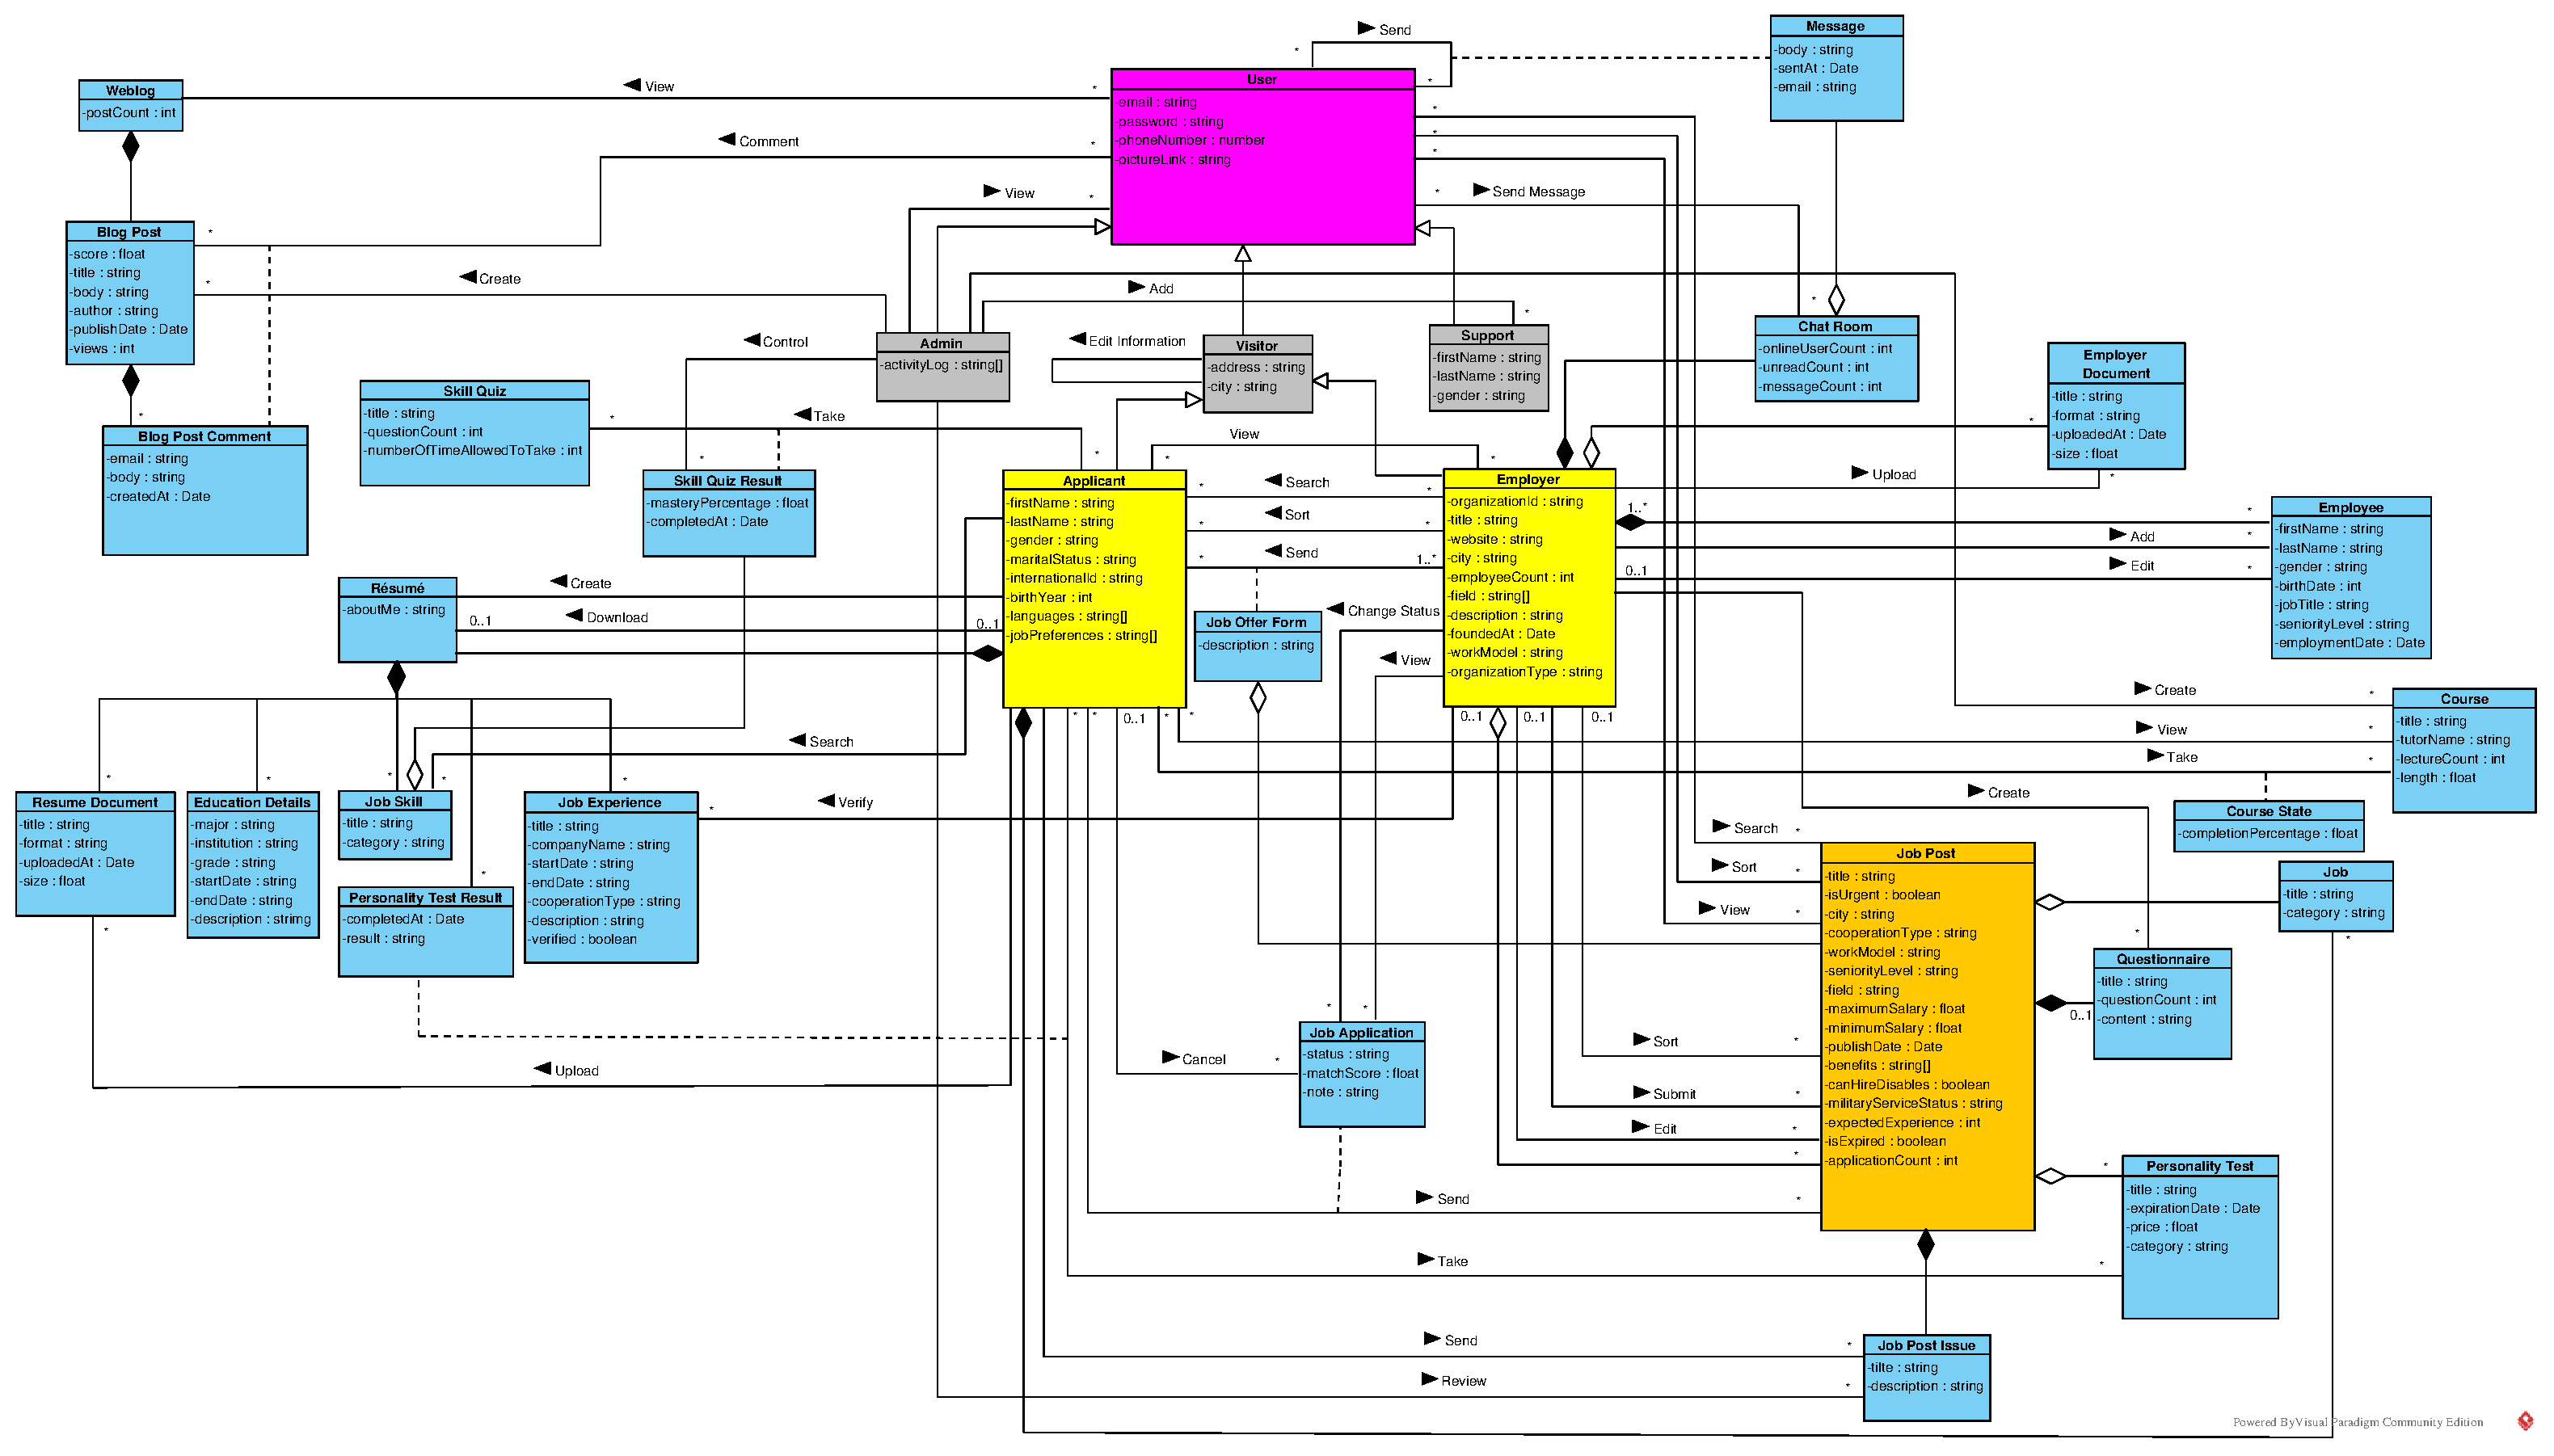
\includegraphics[width=1.5\linewidth]{files/Project_OOAD_Phase2_DiagramClass_V5_EnglishVersion}
		\caption{}
		\label{fig:projectooadphase2diagramclassv5englishversion}
	\end{figure}

	\newpage
	\section{مدل‌سازی دامنه}
	\newpage
	\section{طراحی معماری}

	\newpage
	\section{استخراج موردکابردها و مدل‌سازی تعامل کنشگر-سیستم}

	\begin{itemize}
		\item First item
		\item Second item
		\item Third item
	\end{itemize}

	\begin{enumerate}
		\renewcommand{\labelenumi}{.R\arabic{enumi}}
		\item First item
		\item Second item
		\begin{enumerate}
			\renewcommand{\labelenumii}{.R\arabic{enumi}.\arabic{enumii}}
			\item First subitem
			\item Second subitem
		\end{enumerate}
		\item Third item
	\end{enumerate}


\end{document}